Weiterhin können wir durch nachrechnen diese weiteren Eigenschaften überprüfen:
\begin{enumerate}
    \item
    $\rot F = \rot (F + \tilde{F}) $, falls $\tilde{F} = 
    \div g $  ein Gradientenfeld ist.
    \item
    $\div F = \div (F + \tilde{F}) $, falls $\tilde{F} = 
    \rot G $ ein Rotationsfeld ist.
\end{enumerate}

\begin{definition}[Kohärente Orientierung]
\mbox{}\\
Sei $M \subset \mathbb{R}^3 $ eine 2-dimensionale Mannigfaltigkeit mit dem ENF $\nu $
und sei $W \subset M $ offen bezüglich $M$, 
$\partial_M W $ bezeichne den Rand von $W$ bezüglich $M$.

\begin{center}
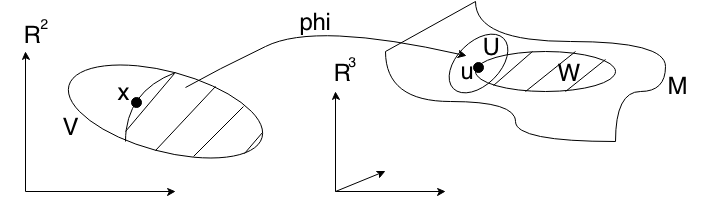
\includegraphics[scale=0.4]{pictures/009-01.png}
\end{center}

Ein Randpunkt $u \in \partial_M W $ heißt \textbf{regulär}, falls für ein Kartengebiet $U$
und eine zugehörige Parametrisierung $\varphi$ der Punkt $x = \varphi^{-1} (u) $
ein regulärer Randpunkt von $\varphi^{-1} (U \cap W) \subset \mathbb{R}^2 $ ist.\\
(Da ein Kartenwechsel ein Diffeomorphismus ist, ist diese Definition unabhängig vom
speziellen $\varphi$.)

$W \subset M $ hat einen \textbf{glatten Rand} $\partial_M W $ bezüglich $M$
falls alle  $u \in \partial_M W $ regulär sind.\\
In diesem Fall ist $\partial_M W $ eine 1-dimensionale Mannigfaltigkeit.\\
(Denn $\varphi$ auf $\varphi^{-1} (\partial_M W \cap U) $ 
ist die zugehörige Parametrisierung\\
und $\varphi^{-1} (\partial_M W \cap U) $ ist eine 1-dimensionale Mannigfaltigkeit.)

Somit ist $\partial_M W $ lokal als reguläre Kurve darstellbar und eine Einheitstangente
$t(u) $ exisitiert.\\
$t: \partial_M W \rightarrow \mathbb{R}^3 $ 
\textbf{orientiert} $\partial_M W $ \textbf{kohärent} zu $M$, 
falls $t(u) $ der Tangenteneinheitsvektor an $\partial_M W \ \forall u $ und
eine stetige Abbildung ist und 
$\nu(u) \times t(u) \in T_u M $ für alle $u$ 'zur Menge $W$ zeigt'.
(Man sagt auch, $W$ liegt 'links vom Rand'.)

\begin{center}
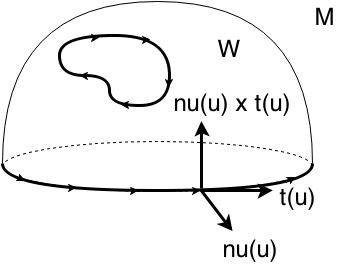
\includegraphics[scale=0.5]{pictures/009-02.png}
\end{center}

\end{definition}

\begin{satz}[Integralsatz von Stokes - klassisch im $\mathbb{R}^3 $]
\mbox{}\\
Sei $F: \Omega \subset \mathbb{R}^3 \rightarrow \mathbb{R}^3 $,
$\Omega$ offen, ein $C^1$-Vektorfeld;
sei $M \subset \Omega $ eine 2-dimensionale Mannigfaltigkeit, orientiert,
mit dem ENF $\nu$ und sei $W \subset M $ beschränkt,
mit glattem Rand $\partial_M W $ welcher mit $t$ zu $M$ kohärent orientiert ist. Dann gilt:

\begin{equation}
    \int\limits_W \rot F(u) \cdot \nu(u) \mathrm{d}a
    =
    \int\limits_{\partial_M W} F(u) \cdot t(u) \mathrm{d}a
\end{equation}

\end{satz}

Das heißt das Integral über die Wirbel des Vektorfelds $F$ 'in der Fläche' $W$\\
(d.h.  $\nu \cdot \rot F $)
ist gleich der Zirkulation von $F$ entlang des Randes $\partial_M W $.

\begin{proof}

$W$ möge im Kartengebiet $U$ von $M$ liegen (sonst ZdE nötig),
die zugehörige Parametrisierung sei $\varphi: V \subset \mathbb{R}^2 \rightarrow U $,
die Koordinate $x = (x_1, x_2) $ liegt in $V$, 
$u = (u_1, u_1, u_3) $ in $M$ bzw. $\Omega$.
$G$ sei $\varphi^{-1} (W) \subset V $, offen und beschränkt mit glattem Rand $\partial G $.

Man will nun (32.16) auf den Gaußschen Satz in $G \subset \mathbb{R}^2 $ zurückführen.

Zunächst hat man:

\begin{equation*}
\nu(\varphi(x)) = 
\frac
    {\pdiff{\varphi}{x_1} (x) \times \pdiff{\varphi}{x_2} (x)}
    {\left| \pdiff{\varphi}{x_1} (x) \times \pdiff{\varphi}{x_2} (x) \right|}
\end{equation*}
(Vergleiche Bsp 29.12: $a \wedge b \stackrel{\mathbb{R}^3}{=} a \times b $) und

\begin{equation*}
\sqrt{\mathrm{det } \varphi'(x)^T \varphi'(x)}
=
\left| \pdiff{\varphi}{x_1} (x) \times \pdiff{\varphi}{x_2} (x) \right| 
\end{equation*}
(vgl. 30.1, 30.2)

Als Integral auf der Mannigfaltigkeit $W$ ist somit die linke Seite in (32.16):

\begin{equation*}
\int\limits_W \rot F(u) \cdot \nu(u) \mathrm{d}a =
\end{equation*}
\begin{equation*}
\stackrel{\text{Def.}}{=}
\int\limits_g \mathrm{rot_u } \ F(\varphi(x)) 
\frac
    {\pdiff{\varphi}{x_1} (x) \times \pdiff{\varphi}{x_2} (x)}
    {\left| \pdiff{\varphi}{x_1} (x) \times \pdiff{\varphi}{x_2} (x) \right|}
\sqrt{\mathrm{det } \varphi'(x)^T \varphi'(x)}
\mathrm{d}x =
\end{equation*}
\begin{equation*}
=
\int\limits_G \mathrm{rot_u } \ F(\varphi(x)) \cdot 
\pdiff{\varphi}{x_1} (x) \times \pdiff{\varphi}{x_2} (x)
\mathrm{d}x = ...
\end{equation*}
\leftskip=30pt Wir nutzen im Folgenden zwecks Kompaktheit folgende Notation:\\
\begin{equation*}
F_l^k \coloneqq \pdiff{F_k}{u_l},\
\varphi_l^k \coloneqq \pdiff{\varphi_k}{x_l} \ \mathrm{wobei\ }\varphi = (\varphi_1, \varphi_2, \varphi_3)
\end{equation*}

\leftskip=0pt
\begin{equation*}
...=
\int\limits_G
\begin{pmatrix}
    F_2^3 - F_3^2 \\
    F_3^1 - F_1^3 \\
    F_1^2 - F_2^1 \\
\end{pmatrix}
\cdot
\begin{pmatrix}
    \varphi_1^2 \varphi_2^3 - \varphi_1^3 \varphi_2^2\\
    \varphi_1^3 \varphi_2^1 - \varphi_1^1 \varphi_2^2\\
    \varphi_1^1 \varphi_2^2 - \varphi_1^2 \varphi_2^1\\
\end{pmatrix}
\end{equation*}

Um weitere Schreibarbeit zu sparen, beschränken wir uns nun auf die die Terme mit $F^1$. Für $F^2$ und $F^3$ sieht das ganze 
völlig analog aus.

\begin{equation*}
    =
    \int\limits_G F_1^1 \cdot 0
    +
    F_2^1 (\varphi_1^2 \varphi_2^1 - \varphi_1^1 \varphi_2^2)
    +
    F_3^1 (\varphi_1^3 \varphi_2^1 - \varphi_1^1 \varphi_2^3)
    +
    \ldots \mathrm{d}x
    \tag{$\heartsuit$}
\end{equation*}

Für die rechte Seite in (32.16) sei

\begin{equation*}
x \rightarrow \tilde{x}(s) = (\tilde{x}_1 (s), \tilde{x}_2 (s))
\end{equation*}
die Parametrisierung der 1-dim. Mf $\partial G $ mit
$s \in I \subset \mathbb{R}$. Dann ist $s \rightarrow \psi(s) \coloneqq \varphi(\tilde{x}(s)) $ die Parametrisierung der 1-dim. Mf $\partial_M W $
und \\
\begin{equation*}
	t(\psi(s)) = \frac{\psi'(s)}{|\psi'(s)|}
\end{equation*}
\begin{equation*}
\psi'(s) = \varphi`(\tilde{x}(s)) \cdot \tilde{x}(s)
\end{equation*}
Dann folgt
\begin{equation*}
    \int\limits_{\partial_M W} F \cdot t \mathrm{d}a
\stackrel{\text{Def.}}{=}
    \int\limits_I F(\psi(s)) \cdot t(\psi(s))
    \underbrace{
        \sqrt{\det \varphi'(s)^T \varphi'(s)}
        }_{
        |\psi'(s)|
        }
    \mathrm{d}s
=
\end{equation*}
\begin{equation*}
    = \int\limits_I F(\varphi(\tilde{x}(s))) \cdot
    \left(
        \varphi'(\tilde{x}(s)) 
        \underbrace{
            \frac{
                \tilde{x}'(s)
                }{
                |\tilde{x}'(s)|
                }
            }_{
            \coloneqq \tilde{t}(\tilde{x}(s))
            }
    \right)
    |\tilde{x}'(s)| \mathrm{d}s = 
\end{equation*}
\begin{equation*}
=
    \int\limits_{\partial G} F (\varphi(x)) \cdot
    \left(
        \varphi'(x) \cdot \tilde{t}(x)) \mathrm{d}s
    \right) = ...
\end{equation*}

\hspace{30pt}
    $
    \tilde{\nu}(\tilde{x}(s))
    =
    \frac{1}{
    | \tilde{x}(s) |}
    \begin{pmatrix}
        \tilde{x}_2'(s) \\
        \tilde{x}_1'(s) \\
    \end{pmatrix}
    $
    ist die äußere Einheitsnormale in $\tilde{x}(s) \in \partial G $ an $G$

\begin{equation*}
...=
    \int\limits_{\partial G} F^1(\varphi(x))
    \left(
        \varphi_1^1 \tilde{x}_1' + \varphi_2^1 \tilde{x}_2'
    \right)
    \frac{1}{| \tilde{x}' |}
    + \ldots \mathrm{d}a = 
\end{equation*}

\begin{equation*}
=
    \int\limits_G F^1(\varphi(x))
    \begin{pmatrix}
        \varphi_2^1(x) \\
        -\varphi_1^1(x) \\
    \end{pmatrix}
    \tilde{\nu}
    + \ldots \mathrm{d}a = 
\end{equation*}
    
\begin{equation*}
\stackrel{\textbf{Gauß}}{=}
    \int\limits_G \mathrm{div_x } \ F^1(\varphi(x))
    \begin{pmatrix}
        \varphi_2^1(x) \\
        -\varphi_1^1(x) \\
    \end{pmatrix}
    + \ldots \mathrm{d}x = 
\end{equation*}
\begin{equation*}
=
    \int\limits_G 
    \mathrm{div_u } \ F^1 \pdiff{\varphi}{x_1} \varphi_2^1(x)
    + \underbrace{F_1 \varphi_{21}^1}_{\text{Schwarzscher Satz}}
    - \mathrm{div_u } \ F^1 \pdiff{\varphi}{x_2} \varphi_1^1
    - \underbrace{F^1 \varphi_{12}^1}_{\sum = 0}
    + \ldots \mathrm{d}x = 
\end{equation*}
\begin{equation*}
=
    \int\limits_G F_1^1 
    \underbrace{\left( \varphi_1^1 \varphi_2^1 - \varphi_2^1 \varphi_1^1 \right)}_{=0}
    + F_2^1 \left( \varphi_1^2 \varphi_2^1 - \varphi_2^2 \varphi_1^1 \right)
    + F_3^1 \left( \varphi_1^3 \varphi_2^1 - \varphi_2^3 \varphi_1^1 \right)
    + \ldots \mathrm{d}x
\end{equation*}

Vergleich mit($\heartsuit$) liefert die Behauptung aus (32.16).

\end{proof}

Nachdem wir uns nun mit Rotation und Divergenz von Feldern auskennen, können wir kurz auf den Hauptsatz der Vektoranalysis 
eingehen, den wir jedoch im Rahmen dieser Vorlesung nicht 
weiter behandeln.\\
\linebreak
\textbf{Einschub: Hauptsatz der Vektoranalysis}\\
Falls für ein unbekanntes Vektorfeld
$F: \Omega \subset \mathbb{R}^3 \rightarrow \mathbb{R}^3 $
die Quellen, die Wirbel und der Fluss durch den Rand bekannt sind, das heißt, gilt für gegebene Funktionen $f: \Omega \rightarrow \mathbb{R}, \ G: \Omega \rightarrow \mathbb{R}^3, \ 
\varphi: \partial \Omega \rightarrow \mathbb{R} $:
\begin{equation*}
\div F = f, \ \rot F = G\ \mathrm{auf\ }\Omega
\end{equation*}
\begin{equation*}
\ F \cdot \nu = \varphi\ \mathrm{auf\ } \partial \Omega 
\end{equation*}

und die Kompatibilitätsbedingungen: 
\begin{equation*}
\div G = 0 \ \mathrm{auf\ }\Omega
\end{equation*} 

\begin{equation*}
\int\limits_{\Omega} f \mathrm{d}x 
= 
\int\limits_{\partial \Omega} \varphi \mathrm{d}a
\end{equation*}
so ist $F $, falls $\Omega,\ f, \ G, \ \varphi $ hinreichend regulär sind, eindeutig bestimmt. \\
Wichtige Anwendungen dessen finden sich z.B. in der Elektrodynamik.


\section{Gradientenfelder}

\begin{definition}[Gradientenfeld]
\mbox{}\\
Eine Abbildung $F: \Omega \subset \mathbb{R}^n \rightarrow \mathbb{R}^n $,
$\Omega $ offen, heißt \textbf{Gradientenfeld},
falls eine differenzierbare Funktion $f: \Omega \rightarrow \mathbb{R} $ exisitiert,
die 
\begin{equation*}
F(x) = f'(x) \ \ \ \forall x \in \mathbb{R} 
\end{equation*}
erfüllt.
\end{definition}
Wir wollen untersuchen, welche Vektorfelder Gradientenfelder sind, analog zur Suche
nach Stammfunktionen in Kapitel 25.

\begin{satz}[Notwendige Bedingung]

Sei $F = (F_1, \ldots, F_n): \Omega \subset \mathbb{R}^n \rightarrow \mathbb{R}^n$,
$\Omega $ offen, stetig differenzierbar und ein Gradientenfeld, 
dann gilt
\begin{equation} 
    \pdiff{}{x_j} F_i (x) = \pdiff{}{x_i} F_j (x) \ \forall x \in \mathbb{R}^n; \
    i,j = 1, \ldots, n
\end{equation}
(31.1) heißt \emph{Integrabilitätsbedingung}; $\pdiff{F_i}{x_j} = \pdiff{f}{x_i x_j} $\\
\linebreak
\emph{Anmerkung:} Für $n=3 $ ist (32.1) äguivalent dazu, dass $\rot F = 0 $ ist.
\end{satz}

